\section{Mating Without Corners: Tablebases}\label{sec:tb}

Up to now our boards have held only kings and pawns. Here we bring in the pieces and ask a classical
question: without corners, which material can still force mate? We computed every
4-man pawnless tablebase on the plane (the ordinary board), on the cylinder (files a and h adjacent) and on the torus (ranks 1
and 8 adjacent as well). Chess on these boards is an old variant~\cite{Pritchard}, but we found no earlier
tablebase for them.

\emph{Rules.} Every piece moves as usual and wraps round each glued edge. A rook, bishop or queen stops when
its ray comes back to its own square, so a rook on an empty rank cannot travel round it and ``pass''. There
is no castling and no fifty-move rule. Stalemate and bare kings are draws, and when black captures, play
continues in the smaller table. A position is legal when the kings are not adjacent, across the seams
included, and the side not to move is not in check. Both sides of the board have even length, so the
coloring of the squares survives the gluing, and ``bishops on opposite colors'' still makes sense.

\emph{Verification.} Two retrograde solvers, written independently from these rules, agree on every position
of all 24 tables, about 607 million values with either side to move \lab{C2}. One of them also re-derives
every value from its children and checks the board's symmetries on every position. On the plane both
reproduce the known longest mates: KQK 10, KRK 16, KBBK 19 and KBNK 33 moves.

\begin{table}[!t]
\centering
\caption{Four-Man Pawnless Endings: Share Won With White to Move and Longest Forced Mate in Moves
\lab{C2}. KBBK Has Bishops on Opposite Colors}
\label{tab:tb}
\footnotesize
\setlength{\tabcolsep}{4.5pt}
\begin{tabular}{@{}lrrrrrr@{}}
\toprule
& \multicolumn{2}{c}{Plane} & \multicolumn{2}{c}{Cylinder} & \multicolumn{2}{c}{Torus} \\
\cmidrule(lr){2-3}\cmidrule(lr){4-5}\cmidrule(l){6-7}
Material & Won (\%) & Mate & Won (\%) & Mate & Won (\%) & Mate \\
\midrule
KQK  & 100    & 10 & 100    & 10 & 0      & --- \\
KRK  & 100    & 16 & 2.80   & 3  & 0      & --- \\
KBBK & 99.98  & 19 & 100    & 14 & 0      & --- \\
KBNK & 99.51  & 33 & 0.0245 & 2  & 0      & --- \\
KNNK & 0.0107 & 1  & 0.0077 & 1  & 0      & --- \\
KRBK & 100    & 16 & 99.74  & 13 & 0.0218 & 1   \\
KRRK & 100    & 7  & 100    & 8  & 100    & 7   \\
KQRK & 100    & 6  & 100    & 5  & 100    & 5   \\
\bottomrule
\end{tabular}
\end{table}

\begin{figure}[!t]
\centering
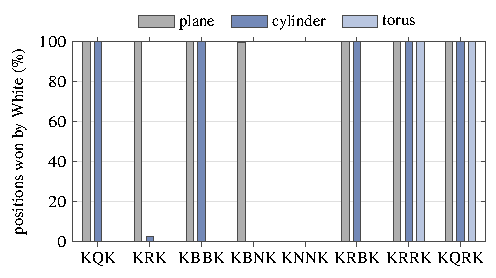
\includegraphics[width=\columnwidth]{figures/tb_bars.pdf}
\caption{Share of legal positions won by white with white to move, for each 4-man pawnless ending on the
plane, the cylinder and the torus (Table~\ref{tab:tb}). On the torus only KRRK and KQRK win; the KRBK
bar (0.0218\%) is too small to see.}
\label{fig:tb_bars}
\end{figure}

Table~\ref{tab:tb} and Fig.~\ref{fig:tb_bars} give the results. The queen does not notice the seam: KQK
is won from every position on the cylinder, in at most 10 moves, as on the plane. The rook and the minor pieces
do notice it.

\emph{KRK and KBNK are draws on the cylinder.} The first and eighth ranks are still edges, but each is now a
closed loop with no corner in it. The rook wins only 2.80\% of the positions, all of them mates in at most
three moves. The longest is Ka3, Rb2 against Ka1: 1.~Rb3 Kh1 2.~Rg3 Ka1
3.~Rg1\#. On the cylinder h1 and h2 are neighbors of a1, so the rook covers h1 along the first rank and the
white king covers h2 across the seam. The bishop and knight win only 0.0245\% of the positions, within two
moves; on the plane their mate needs a corner of the bishop's color, and the cylinder has none.

\emph{Bishops on opposite colors win every position on the cylinder}, in at most 14 moves against 19 on
the plane. Here the seam helps the attacker: a diagonal winds round the cylinder, so from every square of the
first rank a bishop reaches the eighth. The longest line ends in Ke6, Be1, Bf1 against Ke8. The bishop on f1
gives check along f1--h3--a4--e8, once round the board, and the bishop on e1 covers d8 and f8 along its two diagonals.

\emph{On the torus no single piece, and no pair weaker than two rooks, can force mate.} KQK, KRK, KBBK, KBNK and KNNK
are not won from a single position. KRBK wins 0.0218\% of the positions, and every one of these wins is a
mate in one. The bishop pair even has mating positions on the torus, but none of them can arise from a
legal white move. Only KRRK and KQRK win, from every position.

\subsection{King and Pawn Against King}\label{sec:kpk}

We solved every legal KPK position on the $8\times8$ plane and cylinder twice: with the king-and-pawn solver
used for the tr\'ebuchet (all four promotions) and with a separately written KPK solver (queen promotion
only). On the cylinder the two agree on all 326,640 positions. On the plane they differ on exactly 6, the
positions in which only promotion to a rook avoids stalemate, such as Ka4, Pb7 against Ka6 \lab{C2}.
Table~\ref{tab:kpk} gives the counts and Fig.~\ref{fig:kpk_bars} the shares won. The cylinder has fewer
legal positions because the kings may not stand next to each other across the seam.

\begin{table}[!t]
\centering
\caption{King and Pawn Against King: Legal Positions and white Wins on the $8\times8$ Plane and Cylinder
\lab{C2}}
\label{tab:kpk}
\footnotesize
\begin{tabular}{@{}lrrrr@{}}
\toprule
& \multicolumn{2}{c}{White to move} & \multicolumn{2}{c}{Black to move} \\
\cmidrule(lr){2-3}\cmidrule(l){4-5}
Board & Legal & White wins & Legal & White wins \\
\midrule
Plane    & 163,328 & 124,960 & 168,024 & 97,604 \\
Cylinder & 160,656 & 126,736 & 165,984 & 92,760 \\
\bottomrule
\end{tabular}
\end{table}

\begin{figure}[!t]
\centering
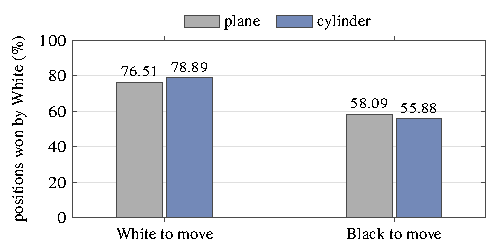
\includegraphics[width=\columnwidth]{figures/kpk_bars.pdf}
\caption{Share of legal KPK positions won by white, plane against cylinder, with white and with black to
move (Table~\ref{tab:kpk}). The seam raises white's share with white to move and lowers it with black to
move.}
\label{fig:kpk_bars}
\end{figure}

\begin{figure}[!t]
\centering
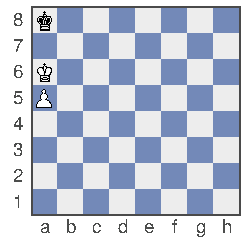
\includegraphics[width=0.5\columnwidth]{figures/kpk_rookpawn.pdf}
\caption{Ka6, Pa5 against Ka8 (cylinder: files a and h adjacent). White wins with either side to move. On
the ordinary board it is the rook-pawn draw with either side to move.}
\label{fig:kpk_rookpawn}
\end{figure}

On a cylinder every file is a center file, so there are no rook pawns.
Fig.~\ref{fig:kpk_rookpawn} shows the classic rook-pawn draw: on the plane the black king cannot be driven
out of the corner without stalemate. On the cylinder we may shift every man four files to the right, and
the position becomes Ke6, Pe5 against Ke8, the textbook win, whoever is to move, with the king on the sixth rank in
front of its pawn. Back on the a-file, with black to move, play goes 1\ldots~Kb8 2.~Kh7! Kb7 3.~a6+, and the pawn
promotes under the king, which guards a7 and a8 from h7 across the seam.

Of the 326,640 positions legal on both boards, 16,538 flat draws become cylinder wins, among them
that of Fig.~\ref{fig:kpk_rookpawn}. The seam also
helps the defender, since a king on the h-file now stands beside an a-pawn: 15,930 flat wins become
cylinder draws. Zugzwang, the engine of the tr\'ebuchet, is more common on the cylinder. The cylinder has 216
mutual zugzwangs, positions in which white to move only draws but black to move loses, against 160 on the
plane \lab{C2}.
